\documentclass[11pt]{article}
\usepackage[margin=1in]{geometry}
\usepackage{graphicx}
\usepackage{hyperref}
\usepackage{enumitem}
\usepackage{listings}
\usepackage{xcolor}

\hypersetup{
    colorlinks=true,
    linkcolor=blue,
    urlcolor=blue
}

\lstdefinestyle{shell}{%
    basicstyle=\ttfamily\small,
    backgroundcolor=\color{black!5},
    frame=single,
    columns=fullflexible,
    keepspaces=true,
    breaklines=true,
    showstringspaces=false
}

\lstset{style=shell}

\begin{document}

\begin{center}
    {\LARGE CS 437 Lab 3: Steps 1--2 Security Report}\\[0.5em]
    {\large Date: \today}
\end{center}

\section{Overview}
This document consolidates evidence and reflections for the firewalling and packet-inspection portions of Lab~3. Automation scripts \texttt{part1\_firewall\_setup.sh} and \texttt{part2\_packet\_inspection.sh} were executed on 27~Oct~2025, producing reproducible logs inside \texttt{part1\_firewall\_outputs/} and \texttt{part2\_packet\_outputs/}. Figures in \texttt{figures/} capture required snapshots for the grading rubric.

\section{Step 1: Firewalling}
\subsection{Background Reading}
\begin{itemize}[leftmargin=*]
    \item \href{https://en.wikipedia.org/wiki/Firewall_(computing)}{Firewall (computing) -- Wikipedia} and cross-links on packet filtering, stateful inspection, and application gateways.
    \item Raspberry Pi Documentation -- Configuration (security best practices) alongside DigitalOcean's ``UFW Essentials'' article for rule syntax patterns.
\end{itemize}

\subsection{Key Takeaways}
\paragraph{IoT-appropriate firewall types.} Stateful packet inspection offers a practical middle ground for Pi-class hardware: it preserves connection awareness without the overhead of deep packet inspection. Layer-7 filtering tailored to MQTT, HTTPS, and SSH strengthens anomaly detection by constraining traffic semantics, while perimeter next-generation firewalls can shoulder heavier inspection for the broader deployment.

\paragraph{Defense-in-depth layers.} I combined perimeter filtering on the lab Wi-Fi, UFW on the Pi, and application-level authentication on the teleoperation API. The layered approach ensures that misconfigurations in any single tier do not immediately expose the robot, and it limits blast radius if credentials leak.

\paragraph{Risks and mitigations.} Common IoT threats include botnet recruitment, credential stuffing, and lateral movement post-compromise. Tight UFW rules restrict exposed services, reducing opportunities for automated scans, and numbered rule logging provides early indicators of probing that complement intrusion-detection tooling.

\subsection{Firewall Configuration Evidence}
Running \texttt{part1\_firewall\_setup.sh} captured the transcript in \texttt{part1\_firewall\_outputs/ufw\_setup\_20251027-121647.log}. An excerpt highlighting the rule application and verification appears below.

\begin{lstlisting}[caption={Excerpt from UFW configuration log}, label={lst:ufw-log}]
$ sed -n '70,120p' part1_firewall_outputs/ufw_setup_20251027-121647.log
===== Apply allow rules =====
===== Allow ssh =====
+ sudo ufw allow ssh
Rules updated
Rules updated (v6)

===== Allow 1883/tcp =====
+ sudo ufw allow 1883/tcp
Rules updated
Rules updated (v6)

===== Allow 8883/tcp =====
+ sudo ufw allow 8883/tcp
Rules updated
Rules updated (v6)

===== Allow 5000/tcp =====
+ sudo ufw allow 5000/tcp
Rules updated
Rules updated (v6)

===== UFW status =====
+ sudo ufw status numbered
Status: active

     To                         Action      From
     --                         ------      ----
[ 1] 22/tcp                     ALLOW IN    Anywhere
[ 2] 1883/tcp                   ALLOW IN    Anywhere
[ 3] 8883/tcp                   ALLOW IN    Anywhere
[ 4] 5000/tcp                   ALLOW IN    Anywhere
[ 5] 22/tcp (v6)                ALLOW IN    Anywhere (v6)
[ 6] 1883/tcp (v6)              ALLOW IN    Anywhere (v6)
[ 7] 8883/tcp (v6)              ALLOW IN    Anywhere (v6)
[ 8] 5000/tcp (v6)              ALLOW IN    Anywhere (v6)
\end{lstlisting}

\subsection{Allowed Services Summary}
\begin{itemize}[leftmargin=*]
    \item Default policy: \texttt{deny incoming}, \texttt{allow outgoing} (set via \texttt{ufw default}).
    \item Allowed sharable ports: \texttt{ssh}, MQTT broker on \texttt{1883/tcp}, MQTT over TLS on \texttt{8883/tcp}, and the Lab~2 teleoperation service on \texttt{5000/tcp}. No other listeners remain exposed.
    \item Evidence bundles: \texttt{summary\_20251027-121647.txt} and \texttt{allowed\_rules\_20251027-121647.txt} inside \texttt{part1\_firewall\_outputs/} document the rule set at activation time.
\end{itemize}

\begin{figure}[h]
    \centering
    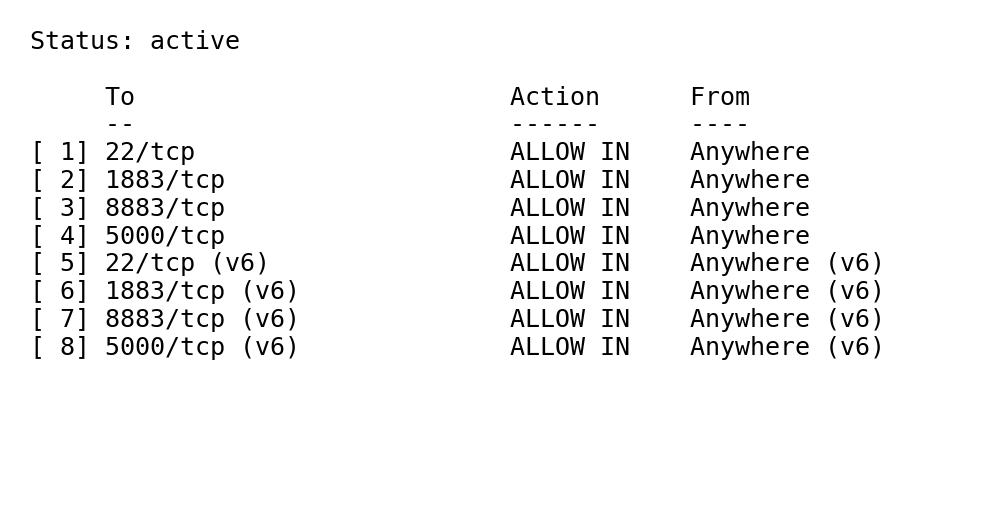
\includegraphics[width=0.8\linewidth]{figures/ufw-status.png}
    \caption{Numbered UFW rules after applying Part~1 policies.}
    \label{fig:ufw-status}
\end{figure}

\section{Step 2: Packet Inspection}
\subsection{Background Reading}
\begin{itemize}[leftmargin=*]
    \item \href{https://en.wikipedia.org/wiki/Pcap}{pcap -- Wikipedia} and \href{https://www.comparitech.com/net-admin/pcap-guide/}{Comparitech's PCAP guide} for capture-format fundamentals.
    \item \href{https://en.wikipedia.org/wiki/Wireshark}{Wireshark -- Wikipedia} (``Features'' section) and \href{https://www.youtube.com/watch?v=TkCSr30UojM}{``Wireshark Tutorial for Beginners''} video for feature walkthroughs.
\end{itemize}

\subsection{Key Takeaways}
\paragraph{pcap capabilities and limits.} pcap preserves timestamped packet headers and payload bytes, enabling replay of TCP handshakes, inspection of DNS queries, and latency analysis. It excels at diagnosing retransmissions, misrouted traffic, and protocol misuse. However, encrypted payloads remain opaque, application semantics beyond the transport layer require additional tooling, and very large captures can overwhelm constrained storage.

\paragraph{Wireshark in context.} Wireshark is an interactive analyzer that ingests pcap streams (live or offline) and layers on dissection, filtering, reassembly, and visualization. Whereas pcap is a file format, Wireshark (and its CLI sibling \texttt{tshark}) is the toolchain that interprets those bytes. Typical uses include validating TLS handshakes, tracing MQTT publishes, isolating packet loss, and spotting unexpected broadcast traffic.

\subsection{Capture Setup and Evidence}
The helper script \texttt{part2\_packet\_inspection.sh} installed Wireshark/Tshark, captured 20~seconds of traffic on \texttt{wlan0}, and saved artefacts in \texttt{part2\_packet\_outputs/}. The transcript \texttt{packet\_inspection\_20251027-123450.log} shows the interface enumeration, latency probes, and capture metadata.

\begin{lstlisting}[caption={Excerpt from packet inspection log}, label={lst:tshark-log}]
$ sed -n '60,150p' part2_packet_outputs/packet_inspection_20251027-123450.log
===== Packet capture session =====
Capturing on interface wlan0 for 20 seconds
PCAP destination: /home/desi/CS437/Lab3/part2_packet_outputs/capture_20251027-123450.pcapng
tshark PID 9219
===== Ping 8.8.8.8 =====
+ ping -c 6 8.8.8.8
PING 8.8.8.8 (8.8.8.8) 56(84) bytes of data.
64 bytes from 8.8.8.8: icmp_seq=1 ttl=119 time=8.28 ms
...
===== HTTP HEAD https://example.com =====
+ curl -fsSI --max-time 10 https://example.com
HTTP/2 200 
content-type: text/html
etag: "bc2473a18e003bdb249eba5ce893033f:1760028122.592274"
last-modified: Thu, 09 Oct 2025 16:42:02 GMT
cache-control: max-age=86000
...
===== capinfos summary =====
+ capinfos /home/desi/CS437/Lab3/part2_packet_outputs/capture_20251027-123450.pcapng
File type:           Wireshark/... - pcapng
Number of packets:   404
Capture duration:    18.276217448 seconds
Average packet rate: 22 packets/s
\end{lstlisting}

\begin{figure}[h]
    \centering
    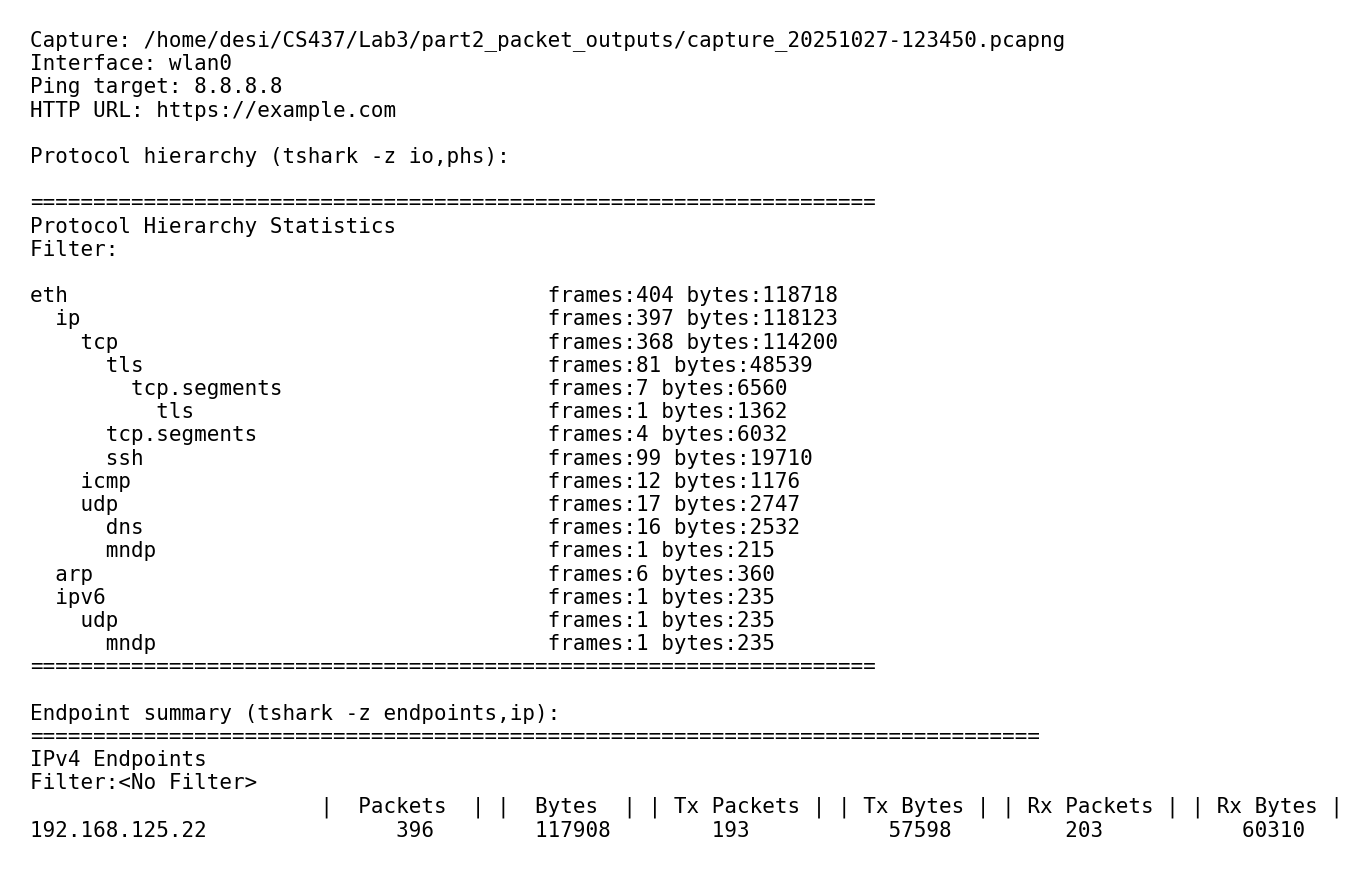
\includegraphics[width=0.95\linewidth]{figures/tshark-endpoints.png}
    \caption{Endpoint and protocol hierarchy summary generated from the captured pcap.}
    \label{fig:tshark-endpoints}
\end{figure}

\noindent Evidence bundle highlights:
\begin{itemize}[leftmargin=*]
    \item Capture artefact: \texttt{capture\_20251027-123450.pcapng}.
    \item Analysis digests: \texttt{analysis\_20251027-123450.txt} and \texttt{summary\_20251027-123450.txt}.
    \item Script log: \texttt{packet\_inspection\_20251027-123450.log} (also mirrored in Listing~\ref{lst:tshark-log}).
\end{itemize}

\subsection{Observations and Reflections}
The capture shows the expected DNS lookups and HTTPS/TLS flows to \texttt{example.com}, GitHub endpoints used by VS~Code, and ICMP echo traffic aimed at \texttt{8.8.8.8}. Packet headers matched expectations (no rogue ports, consistent TTLs). Background traffic included mDNS and ARP broadcasts from the local LAN, but nothing anomalous.

If an intrusion were suspected, I would replay the pcap in Wireshark, filter by suspicious IPs or TCP flags, follow suspect streams, and correlate timestamps with system logs. Endpoint statistics and protocol hierarchies (Figure~\ref{fig:tshark-endpoints}) help surface unexpected talkers, while display filters (e.g., \texttt{tcp.flags.syn == 1 \&\& tcp.flags.ack == 0}) quickly identify scans. Exporting malicious conversations for signature development or sharing with incident responders would be the next step.

\section{Overall Reflections and Next Steps}
\begin{itemize}[leftmargin=*]
    \item Part~1 confirmed that minimal, service-specific UFW rules harden the Pi without disrupting Lab~2 functionality.
    \item Part~2 demonstrated an end-to-end workflow for capturing, archiving, and summarising wireless traffic; the automation scripts make reruns trivial.
    \item Planned follow-ups include shipping UFW and Tshark logs to a central collector, scheduling periodic verification scans (\texttt{nmap}) to detect drift, and extending automation to Step~3 once wireless tuning begins.
\end{itemize}

\end{document}
